\chapter{Konzeption}
% TODO: weiter schreiben
Dieses Kapitel beinhaltet alle Schritte für die Konzeption der angewandte Methoden. Außerdem wird der Datensatz und die verwendeten Tools 
präsentiert.

\section{Image Colorization als Multimodales Problem}
Konventionelle automatische Methoden zielen darauf ab, die Farben für ein generiertes Bild so nah wie möglich an das Originale Bild vorherzusagen.
Diese Methoden verwenden ein MSE Loss der Vorhersagen die Weit von den Originalen Farbwerte entfernt liegen, stärker bestraft, als Farbwerte
die dichter an den Originalen Farbwerte liegen. Das führt, wie bei \ref{subsection:verwandte-arbeiten} beschrieben, zu entsättigte Bilder.
Die Gründe für diese Ergebnisse ist dass verschiedene Objekte, verschiedene Farben einnehmen können. Aus diesem Grund, behandelt die vorliegende
Arbeit das Problem als ein Multimodales Problem.

% TODO: finish this
\section{Farbraum}
Der Standard Farbraum der Bilder für die Methoden dieser Arbeit ist der RGB-Farbraum. Bei diesem Farbraum lässt sich schwer das Graustufen Bild 
von den Farbkanäle zu trennen, daher wird der Lab-Farbraum verwendet.
\\
\\
Bei den Lab-Farbraum können ohne Probleme die Farbkanäle ``ab'' von den Belichtungskanal ``L'' getrennt werden. Der Belichtungskanal ``L'' 
enthält das Graustufenbild die in den CNN eingespeist wird. Das generierte Bild wird für die Darstellung von dem Lab-Farbraum in den RGB-Farbraum 
konvertiert.

\begin{figure}[H]
  \vspace{1cm}
  \centering
  \begin{subfigure}
    \centering
    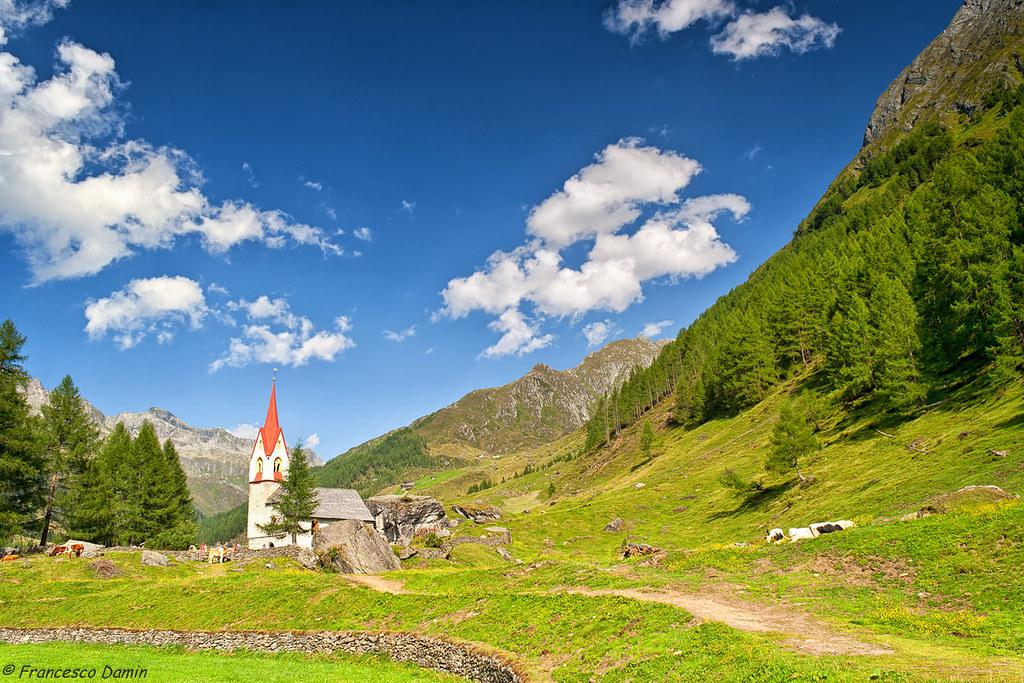
\includegraphics[width=.35\textwidth]{resources/colorspace/image.jpg}
  \end{subfigure}
  \begin{subfigure}
    \centering
    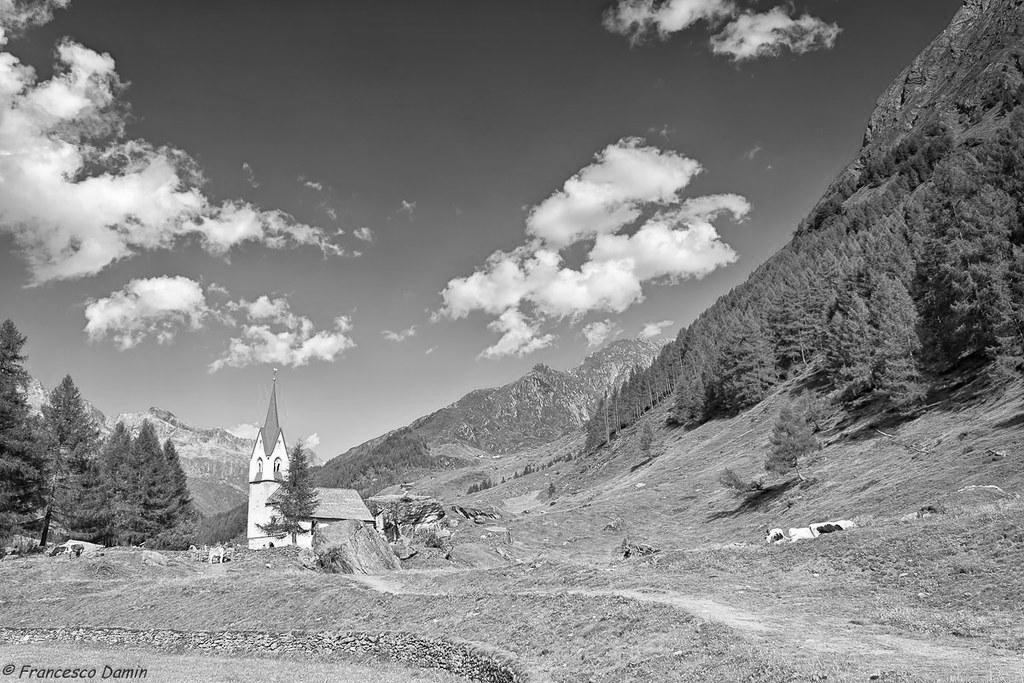
\includegraphics[width=.35\textwidth]{resources/colorspace/grayscale.png}
  \end{subfigure}


  \begin{subfigure}
    \centering
    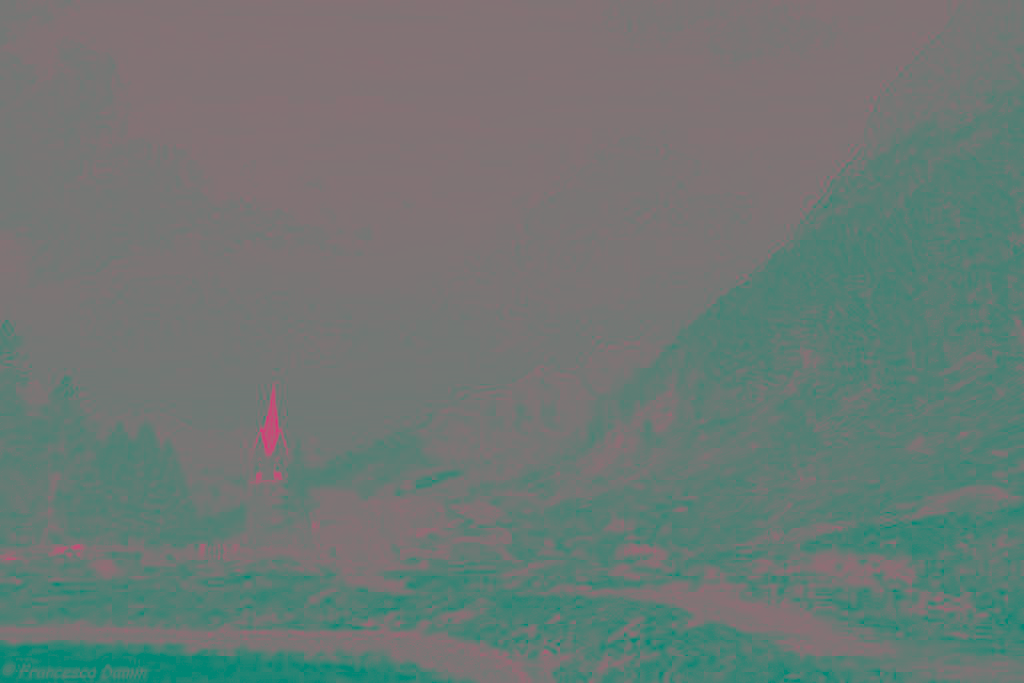
\includegraphics[width=.35\textwidth]{resources/colorspace/a_channel.png}
  \end{subfigure}
  \begin{subfigure}
    \centering
    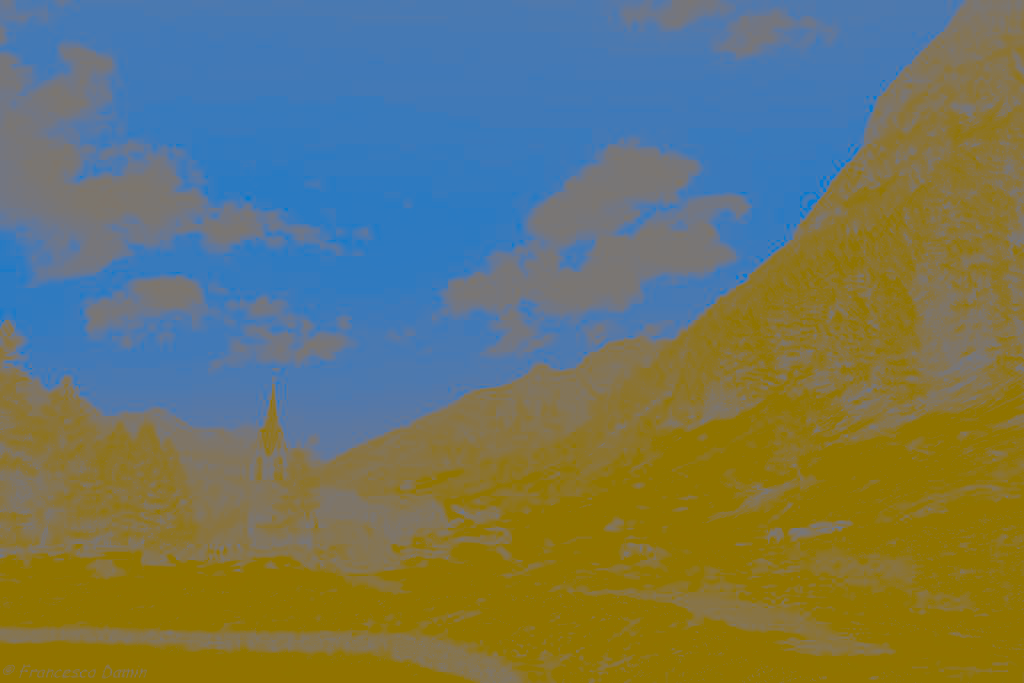
\includegraphics[width=.35\textwidth]{resources/colorspace/b_channel.png}
  \end{subfigure}
  \caption{Originales Bild oben links, den Belichtungskanal ``L'' oben rechts, unten links den Farbkanal ``a'' und unten rechts den Farbkanal ``b''.}
  \label{image:farbraum}
\end{figure}

% TODO: maybe new image
\section{Binning}\label{section:binning}
Binning ist eine Technik, die für die Bildverarbeitung verwendet wird. Binning wird, in dem Kontext von Image Colorization, als Eingruppierung 
von naheliegenden Farben definiert. Die Farben werden in gleich große Intervalle aufgeteilt. Diese Intervalle bezeichnet man im Englischen als
``\gls{bin}s''. Jedes dieser Intervalle wird durch einen \gls{bin} Index repräsentiert, somit reduziert sich die Anzahl der Klassen die vorhergesagt werden
können.

Als Beispiel für die Veranschaulichung wird der normalisierte Lab-Farbraum in 36 gleich große \gls{bin}s unterteilt. Da die Farbinformationen 
in den ``ab'' Farbkanäle kodiert sind, werden nur diese 2 Farbkanäle in \gls{bin}s klassifiziert. Auf dem Bild \ref{image:bins} ist der Farbkanal 
``a'' auf der x-Achse und der ``b'' Farbkanal auf der y-Achse abgebildet. Die Vierecke repräsentieren die \gls{bin}s. Die obere Zahl in den Bins 
symbolisiert die $xy$ Koordinaten auf dem \gls{grid}, die untere unterstrichene Zahl symbolisiert den Bin Index. 
Die $xy$ Koordinaten \gls{grid} sind Bedeutsam für die Berechnung der Bins.

\begin{figure}[H]
  \centering
  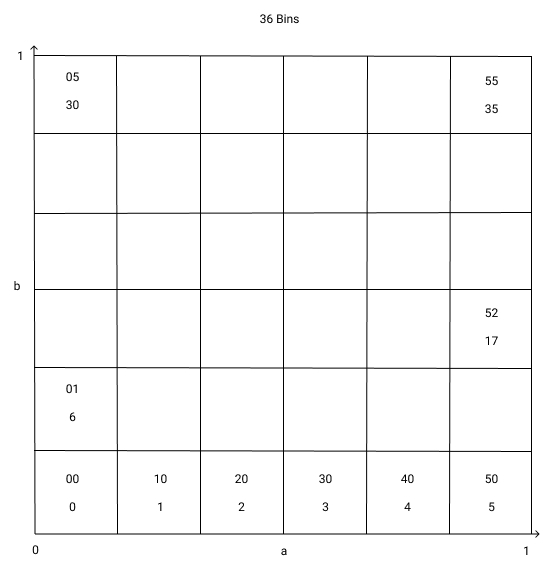
\includegraphics[width=0.65\textwidth]{resources/bins/bins.jpg}
  \caption{
  \gls{grid} mit 36 bins. Die x-Achse bildet die Werte von dem Farbkanal ``a'' und die y-Achse die Werte von den Farbkanal ``b'' ab.
  }
  \label{image:bins}
\end{figure}

Für die Methoden dieser Arbeit wurden nur symmetrische \gls{grid}s verwendet, so ergibt zum Beispiel ein $6 \times 6$ Grid 36 Bins und 
ein $18 \times 18$ Grid 324 Bins.

\subsection{Umwandlung von Bin zu Farbe}
Die Umwandlung von Bin zu Farbe muss für die Ergebnisse von dem Netzwerk ebenfalls vorgegeben sein. Für dieses Problem werden vor dem 
Training die Farben von jedem Pixel aus den Trainingsbildern in Bins klassifiziert. Diese Klassifikation verläuft separat für jeden Farbkanal.
Anschließend wird der Modus und den Durchschnitt pro Farbkanal der unter jedem Bin klassifizierten Farben ausgerechnet. Zuletzt werden die Werte
in zwei separate Dateien gespeichert.

\section{Netzwerkarchitektur}
Die Netzwerkarchitektur ist ein wichtiger Faktor dass u.a. die Ergebnisse beeinträchtigen kann. Wichtig um die Methoden zu vergleichen ist ein
leichtes Netzwerk der wenige Parameter besitzt, schnell zu trainieren ist und gute Ergebnisse liefert. Da mit Bildern gearbeitet wird, eignen sich
Convolutional Neural Networks besonders gut.
\\
\\
Das Ziel von dem Netzwerk ist es, ein Graustufenbild als Input zu bekommen und eine Wahrscheinlichkeitsverteilung über alle Bins per Pixel vorherzusagen.
Das Output Volumen hat die Dimensionen $ W_{Input} \times H_{Input} \times 1 $, wobei $W$ und $H$ die Breite und Höhe von dem Bild sind,
mit einer Wahrscheinlichkeitsverteilung über alle Bins bei jedem Pixel. Dieser Ansatz ist auch bei Image Segmentation Probleme genutzt, wo ein Bild
in das Netzwerk einspeist wird und als Output, wird ein Segmentation map, mit eine Klasse per Pixel, erzeugt. In der Regel hat jeder Klasse eine
bestimmte Farbe und dadurch werden Objekte klassifiziert und getrennt. In dem Fall von Image Colorization bekommt jeder Pixel in dem Output Volumen
eine Wahrscheinlichkeitsverteilung über alle Bins die in einer Farbe umgewandelt wird.
\\
\\
Die Methoden von Zhang et al. \cite{zhang2016colorful} verwenden einen \gls{CNN} das einen Graustufenbild als Input entgegen nimmt und ein Volumen mit
eine Wahrscheinlichkeitsverteilung über alle Bins per Pixel generiert. Diese Netzwerkarchitektur besteht aus Blöcke mit jeweils 2 oder 3 Convolutional
und ReLU Layers, gefolgt von einem Batch Normalisation Layer. Batch Normalisation ist eine Regularisierungstechnik die die Werte in einem Hidden Layer
normalisiert, bevor sie in den nächsten Layer weitergereicht werden. Das Netzwerk hat keine Pooling Layers, alle Änderungen in der Auflösung werden durch
Downsampling oder Upsampling zwischen Blöcke erreicht.
\\
Dieser Netzwerkarchitektur ist sehr schwer für die GPU\footnote{Graphics Processing Unit}, was die Batch Größe und Trainingszeit stark beeinflusst.
\\
\\
Aus diesem Grund richtet sich die Netzwerkarchitektur dieser Arbeit nach der Netzwerkarchitektur von Billaut et al. \cite{billaut2018colorunet}. 
Sie verwenden eine angepasste Version von einem U-net Convolutional Neural Network \cite{ronneberger2015unet}. 

\subsection{U-net}\label{section:u-net}
Ein U-net wird häufig bei Image Segmentation angewendet und ist einer Art Autoencoder mit Skip Connections. Im vergleich zu konventionelle Autoencoder, können
der Encoder und Decoder nicht getrennt voneinander verwendet werden und bei dem Decoder werden Transposed Convolutions, als Upsampling 
Methode, verwendet. Das U-net verfügt außerdem über Skip Connections die ermöglichen fein-granuläre Details in dem Output Volumen zu 
wiederherstellen und helfen mit dem Vanishing Gradient Problem in Backpropagation. Skip Connections konkatenieren bestimmte Layers von dem
Encoder mit Layers von dem Decoder, mit der gleichen Dimensionen.
\\
\\
Ein U-net besteht, wie einem Autoencoder, aus einem Encoder und Decoder Teil. Der Encoder besteht aus sogenannten ``ConvBlocks''. ConvBlocks
bestehen aus 2 Convolutional Layers gefolgt von ReLU und Batch Normalisation. Die ConvBlocks werden gefolgt
von einem Pooling Layer die die Dimensionen von dem Volumen verringern. Der Decoder besteht aus ConvBlocks gefolgt von Transposed Convolutions
die die Dimensionen von dem Volumen wieder vergrößern. Das letzte Layer ist eine $1 \times 1$ Convolutional Layer die das Output Volumen generiert.
Skip Connections konkatenieren ConvBlocks aus dem Encoder mit den Transposed Convolutions aus dem Decoder, die die gleiche Dimensionen haben.

% TODO: maybe change image
\begin{figure}[H]
  \centering
  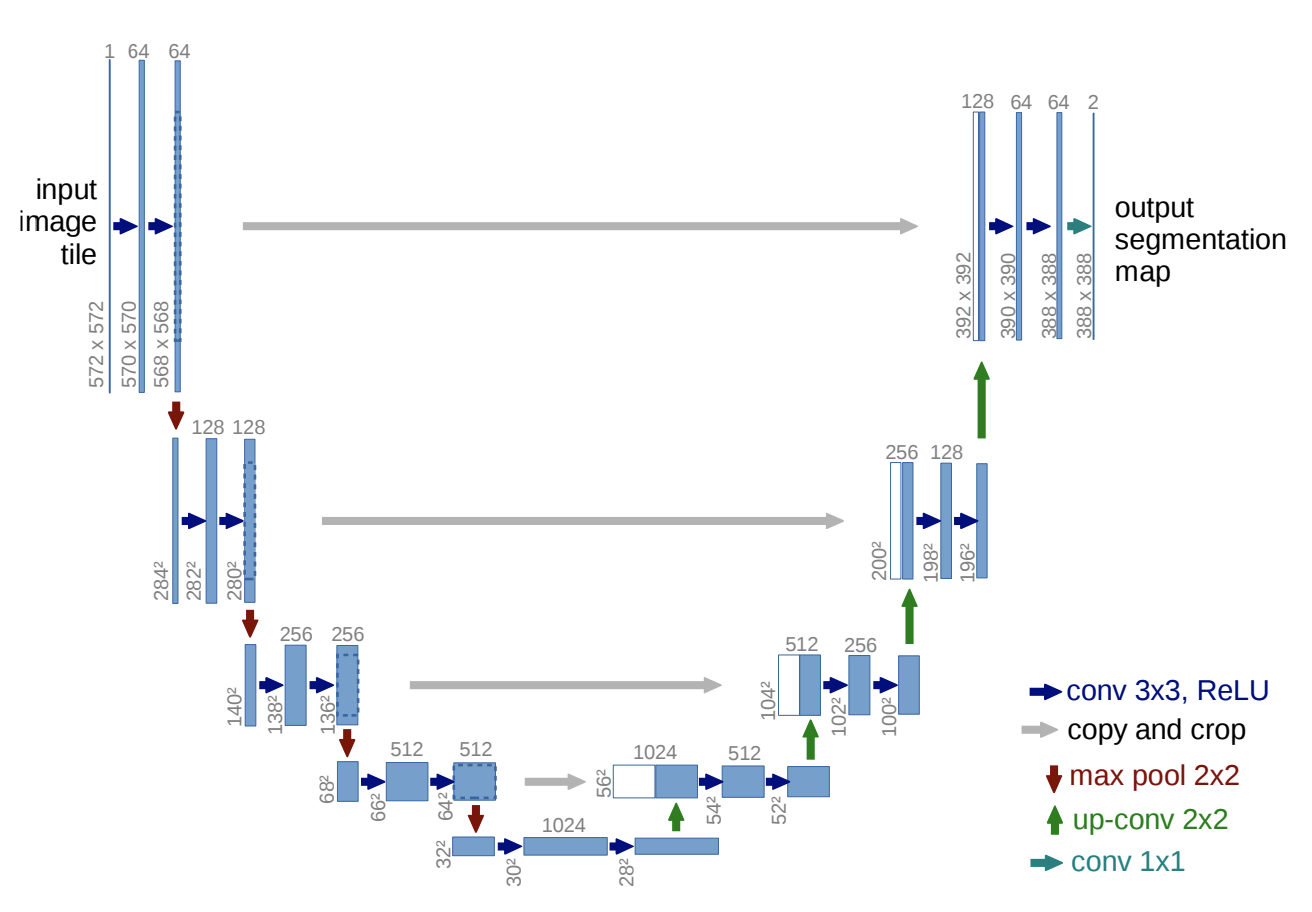
\includegraphics[width=0.85\textwidth]{resources/networks/unet.png}
  \caption{
    U-net Architektur (Beispiel für $32 \times 32$ Pixels in der niedrigste Auflösung). Jeder blaue Box entspricht ein multi-Kanal Feature Map.
    Die Tiefe der Feature Maps ist gekennzeichnet durch die Zahl über die Box. Die Breite und Höhe ist durch die Zahl unten links erkennbar.
    Die weiße Boxen repräsentieren die kopierte Feature Maps. Die Pfeile bestimmen die verschiedene Operationen.
    \cite{ronneberger2015unet}
  }
  \label{image:unet}
\end{figure}

\section{Datensätze}
Um das Netzwerk zu trainieren werden bedeutsame Bilder gebraucht. Ein Vorteil von Image Colorization ist, dass jedes Bild für das Trainieren
verwendet werden kann, da nur die Graustufen Version davon gebraucht wird.

Um die Methode zu prüfen werden 3 Datensätze benutzt, die verschiedene Auflösungen und Themen beinhalten.

Als erstes wird ein Spiel–Datensatz von $ 32 \times 32 $ Bilder generiert. Dieser setzt sich aus 3 geometrischen Objekten und 3 Farben pro
Objekt zusammen. Die geometrischen Objekte sind ein Rechteck, ein Kreis und ein Dreieck pro Bild, die jeweils in eine der 3 Farben eingefärbt sind.
Die Bilder haben einen einheitlichen schwarzen Hintergrund.

\begin{figure}[H]
  \centering
  \vspace{1cm}
  \begin{subfigure}
    \centering
    
\includegraphics[width=.15\textwidth]{resources/dataset/dummy/circle21.png}
  \end{subfigure}
  \begin{subfigure}
    \centering
    
\includegraphics[width=.15\textwidth]{resources/dataset/dummy/circle68.png}
  \end{subfigure}
  \begin{subfigure}
    \centering
    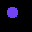
\includegraphics[width=.15\textwidth]{resources/dataset/dummy/circle71.png}
  \end{subfigure}

  \begin{subfigure}
    \centering
    
\includegraphics[width=.15\textwidth]{resources/dataset/dummy/rectangle32.png}
  \end{subfigure}
  \begin{subfigure}
    \centering
    
\includegraphics[width=.15\textwidth]{resources/dataset/dummy/rectangle46.png}
  \end{subfigure}
  \begin{subfigure}
    \centering
    
\includegraphics[width=.15\textwidth]{resources/dataset/dummy/rectangle66.png}
  \end{subfigure}

  \begin{subfigure}
    \centering
    
\includegraphics[width=.15\textwidth]{resources/dataset/dummy/triangle41.png}
  \end{subfigure}
  \begin{subfigure}
    \centering
    
\includegraphics[width=.15\textwidth]{resources/dataset/dummy/triangle49.png}
  \end{subfigure}
  \begin{subfigure}
    \centering
    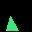
\includegraphics[width=.15\textwidth]{resources/dataset/dummy/triangle51.png}
  \end{subfigure}
  \caption{Beispiel von Trainingsbildern mit einer der möglichen Farbe pro Klasse}
  \label{image:dummy}
\end{figure}

Der Datensatz besteht aus 2664 Bilder für das Training und 324 Bilder für das Testen.
Dieser Datensatz dient als Beweis für die Methode und hilft bei der Entwicklung und Optimierung des Netzwerks.
\\
\\
Als zweites werden 12 Klassen des CIFAR-100\footnote{https://www.cs.toronto.edu/~kriz/cifar.html} Datensatzes verwendet. CIFAR-100 ist 
ein öffentlich verfügbares Datensatz der von Krizhevsky et al. erstellt wurde. Der Datensatz setzt sich aus 100 Klassen mit jeweils 600 
Bildern pro Klasse, außerdem sind die 100 Klassen in 20 Superklassen grupiert. Der Datensatz wird in 50000 Bilder für das Training und 
10000 Bilder für das Testen aufgeteilt. Einige Beispiele für Klassen sind z.B. \textit{apples}, \textit{palm} oder \textit{bee}. 
Die Bildern haben ebenfalls einer Auflösung von $ 32 \times 32 $.

Da ein Model von Null auf zu trainieren, die jedes Objekt auf dem CIFAR-100 Datensatz richtig erkennt und einfärbt, sehr aufwendig wäre, werden
nur bestimmte Klassen für das Training verwendet. Diese Klassen sind: \textit{apples}, \textit{sunflower}, \textit{rose}, \textit{cloud}, 
\textit{maple\_tree}, \textit{oak\_tree}, \textit{pine\_tree}, \textit{willow\_tree}, \textit{palm\_tree},
\textit{mountain}, \textit{forest} und \textit{sea}.
Alle Klassen haben Gemeinsamkeiten, was das erlernen von Merkmale erleichtert im Vergleich zu einem sehr allgemeinen Datensatz.
\\
\\
Abschließend wird ein komplexeres und hochauflösendes Datensatz verwendet, dass Naturbezogene Bilder enthält. Ziel damit ist, ein Netzwerk zu
trainieren das Bilder aus Natur einfärben kann. Dieser besteht 3 Datensätze aus 
Kaggle\footnote{\url{https://www.kaggle.com/}} und GitHub\footnote{\url{https://github.com/}}. 
Das erste ist das ``Landscape Pictures''\footnote{https://www.kaggle.com/arnaud58/landscape-pictures} Datensatz von Arnaud Rougetet, von diesem
Datensatz werden alle Bilder verwendet. Das zweite Datensatz ist das 
``Landscape Classification''\footnote{https://www.kaggle.com/huseynguliyev/landscape-classification?} von Huseyb Guliyev, hiervon werden nur
die Klassen \textit{forest}, \textit{glacier}, \textit{mountain} und \textit{sea} verwendet. Das letzte Datensatz ist das ``Landscapes dataset''
\footnote{https://github.com/ml5js/ml5-data-and-models/tree/master/datasets/images/landscapes} von ml5js auf GitHub. Von diesem Datensatz wurden
die Klassen \textit{field}, \textit{forest}, \textit{lake}, \textit{mountain} und \textit{road} verwendet.
\\
Das fertige Datensatz besteht aus 8 Klassen und hat insgesamt
13363 Bilder, 10945 für das Training und 2409 für das Testen. Die 8 Klassen sind: \textit{field}, \textit{forest}, \textit{glacier}, 
\textit{lake}, \textit{mountain}, \textit{road}, \textit{sea} und ``ohne Kategorie''. 
Die Klasse ``ohne Kategorie'' beinhaltet die Bilder aus dem ``Landscape Pictures'' Datensatz. Die Klassen sind für das Training und 
die Methode nicht relevant, da jedes Pixel in Bins klassifiziert wird. Das finale Datensatz wird ``Landscape Datensatz'' für der Rest der 
Arbeit benannt.

\section{Data Preprocessing und Argumentation}
Für das optimale Training und Ergebnisse werden die Bilder vorverarbeitet. Außerdem werden Techniken von Image Argumentation angewendet.
Das Spiel–Datensatz und die 12 Klassen von CIFAR-100 werden für das Training mit einer Wahrscheinlichkeit von 50\% horizontal gespiegelt.
\\
Da das Landscape Datensatz, Bilder mit verschiedene Auflösungen beinhaltet, werden alle zufällig auf $ 128 \times 128 $ angepasst. Das 
reduziert die Trainingszeit und die Komplexität von dem Datensatz. Für das Training werden die Bilder von diesem Datensatz gleichermaßen mit einer 
Wahrscheinlichkeit von 50\% horizontal gespiegelt. Für die Evaluierung werden die Bilder ebenfalls auf $ 128 \times 128 $ angepasst.

\section{Tools}
Um die Methode zu realisieren werden einige Tools angewendet. Für die Implementierung wird das Framework 
PyTorch\footnote{https://pytorch.org/} angewendet. PyTorch ist ein Open-Source Framework basierend auf Python für Machine Learning und 
Deep Learning. Es wurde von das Facebook AI Research Team entwickelt und erschien im Jahr 2016. Zum Zeitpunkt der Verfassung dieser Arbeit ist 
die Version 1.6.0 die aktuellste. Für die Farbraum Konvertierung wird das ``scikit-image'' Bibliothek eingesetzt.
\\
Das Trainieren von den Modellen wird, wegen den hohen Rechenaufwands, auf zwei verschiedene Plattformen durchgeführt. Die Modelle mit den
$32 \times 32$ Bildern werden auf Google Colab\footnote{https://colab.research.google.com/} trainiert. Google Colab ist eine Plattform von 
Google, die es ermöglicht, Experimente im Browser mit einer Hochleistungsgrafikkarte umzusetzen. Für das Modell mit den $128 \times 128$ Bildern
wird das Curious Containers (CC) Framework\footnote{https://www.curious-containers.cc/} benutzt. Curious Containers ermöglicht eine 
gleichzeitige Durchführung von verschiedene Experimente in einem Cluster von Hochleistungsrechner.


